\documentclass[10pt]{beamer}

%\usepackage[backend=bibtex,firstinits=true,style=verbose-inote,citestyle=authortitle]{biblatex}
\usepackage{bm}
\usepackage{graphicx}
\usepackage{subcaption}
\usepackage{amsmath}
\usepackage{amsfonts}
\usepackage{makecell}
\usepackage{filecontents}
\usepackage{biblatex}
% \newcommand{\expect}[2][]{
\ifthenelse{\equal{#1}{}}{
\mathbb{E}\left[#2\right]
}{
\underset{#1}{\mathbb{E}}\left[#2\right]
}}

\newcommand{\cov}[2][]{
\ifthenelse{\equal{#1}{}}{
\text{Cov}\left[#2\right]
}{
\underset{#1}{\text{Cov}}\left[#2\right]
}}


\newcommand{\var}[2][]{
\ifthenelse{\equal{#1}{}}{
\text{Var}[#2]
}{
\underset{#1}{\text{Var}}[#2]
}}

\newcommand{\loss}[2][]{
\ifthenelse{\equal{#1}{}}{
\mathcal{L}(#2)
}{
\mathcal{L}_{#1}(#2)
}}

\newcommand{\kl}[2]{
\text{D}_\text{KL}[#1 \parallel #2]
}

\newcommand{\R}{\mathbb{R}}
%\newcommand{\Prob}{\mathbb{P}}

\newcommand{\1}[1]{\mathds{1}\{#1\}}


%\usecolortheme{dolphin}
\setbeamertemplate{navigation symbols}{}
\setbeamertemplate{section in toc}{\inserttocsectionnumber.~\inserttocsection}

\begin{filecontents*}{references.bib}
@inproceedings{MultiplicativeOps,
title={Multiplicative Interactions and Where to Find Them},
author={Siddhant M. Jayakumar and Wojciech M. Czarnecki and Jacob Menick and Jonathan Schwarz and Jack Rae and Simon Osindero and Yee Whye Teh and Tim Harley and Razvan Pascanu},
booktitle={International Conference on Learning Representations},
year={2020},
url={https://openreview.net/forum?id=rylnK6VtDH}
}
\end{filecontents*}

\addbibresource{references.bib}


\title{Multiplicative Interactions and Where to Find Them\footnote{\citepaper{MultiplicativeOps}}}
%\subtitle{}
%\author{Ivan Skorokhodov}
%\date{}
%\logo{
\includegraphics[height=1cm]{images/ipavlov-logo.png}}

\newcommand{\citepaper}[1]{\citetitle{#1} by \citeauthor{#1}}

%\graphicspath{{./images}}

%\usetheme{lucid}
\begin{document}

\begin{frame}
    \titlepage
\end{frame}

\begin{frame}{Overview}
    \begin{itemize}
        \item\pause Authors explore scenarios where we fuse two variables $x, z$ ``multiplicatively'', instead of addition (concatenation).
        \item\pause They unify the notions of gating, attention, metric learning, etc by a single notion of \textit{multiplicative interaction} (MI).
        \item\pause They show, that such multiplicative interactions are more \textit{expressive}
        \begin{itemize}
            \item\pause i.e. can represent broader set of functions with smaller amount of parameters.
        \end{itemize}
        %\item MO is much better than concatenation when fusing several streams of information
        \item\pause They achieve SotA performance on several tasks simply by replacing concatenation with MI.
    \end{itemize}    
%    \begin{align*}
%        (z^\top \mathbb{W} x)_k = \sum_{ij} z_i \mathbb{W}_{ijk} x_j = \sum_i z_i \sum_j \mathbb{W}_{ijk} x_j = z^\top (\mathbb{W} x)_k
%    \end{align*}
\end{frame}

\begin{frame}{General definition of Multiplicative Interaction}
Authors define \text{multiplicative interaction} as a function between two variables $x$ and $z$:
\begin{align*}
\mathcal{M}(x, z) = \mathbf{z}^{T} \mathbb{W} \mathbf{x} + \mathbf{z}^{T} \mathbf{U}+\mathbf{V} \mathbf{x}+\mathbf{b},
\end{align*}
where:
\begin{itemize}
    \item $x, z$ are vectors
    \item $\mathbb{W}$ is a 3d-tensor
    \item $U, V$ are 2d-matrices and $b$ is a bias vector.
\end{itemize}
\end{frame}

\begin{frame}{Side note: how to compute $\mathbf{z}^{T} \mathbb{W} \mathbf{x}$}
    \begin{itemize}
        \item\pause $\mathbf{z}^{T} \mathbb{W} \mathbf{x}$ is almost the same as normal product $\mathbf{z}^{T} A \mathbf{x}$
        \item\pause We should just abstract away from what lies in a cell of the matrix
        \item\pause Imagine that each cell of matrix $W$ is an apple
        \item\pause Then $z^\top A x$ produces an apple
        \item\pause Then in case of $\mathbb{W}$ each apple is a 1d-vector
    \end{itemize}
    \begin{figure}
        \centering
        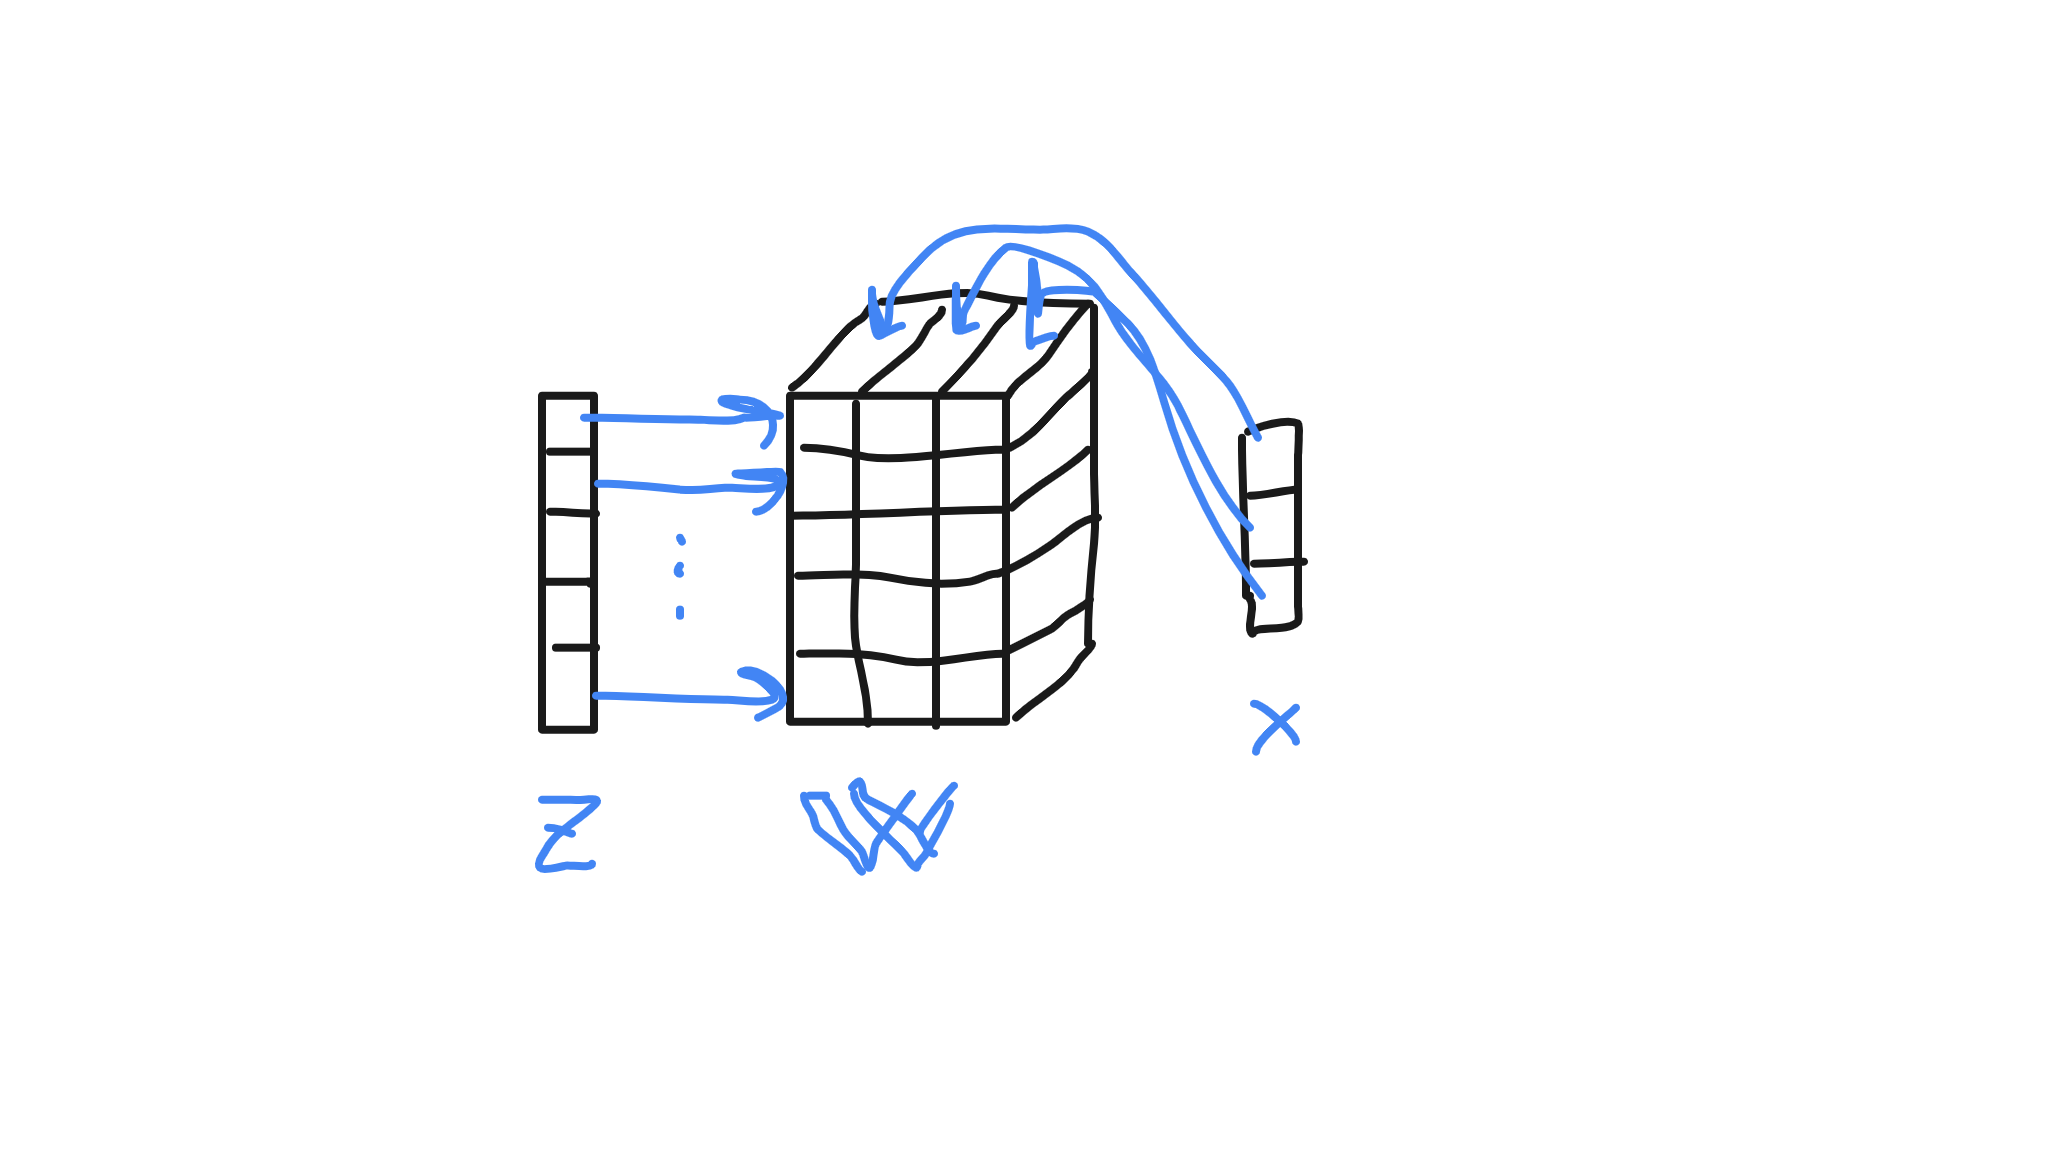
\includegraphics[width=\textwidth]{images/3d-matrix-dot-product}
    \end{figure}
\end{frame}

\begin{frame}{MIs are more expressive}
    \begin{itemize}
        \item\pause It is known, that MLP are \textit{universal approximators}, they can approximate any function with arbitrary small error $\varepsilon$ if they are wide enough.
        \item\pause But they are not able to \textit{represent} any function, i.e. to model it with $\varepsilon = 0$.
        \item\pause \textbf{Definition} Hypothesis space $\mathcal{H}_{f(\theta)}$ is a set of those functions that $f(\theta)$ can represent
        \item\pause \textbf{Theorem}: given an MLP and MI, hypotheses class for MI is \textit{strictly} larger than for MLP.
        \item\pause This means, that MI can represent any function from $\mathcal{H}_\text{MLP}$, but there are some functions that MI can represent, but MLP cannot
    \end{itemize}
\end{frame}

\begin{frame}{MIs are more expressive}
    \begin{figure}
        \centering
        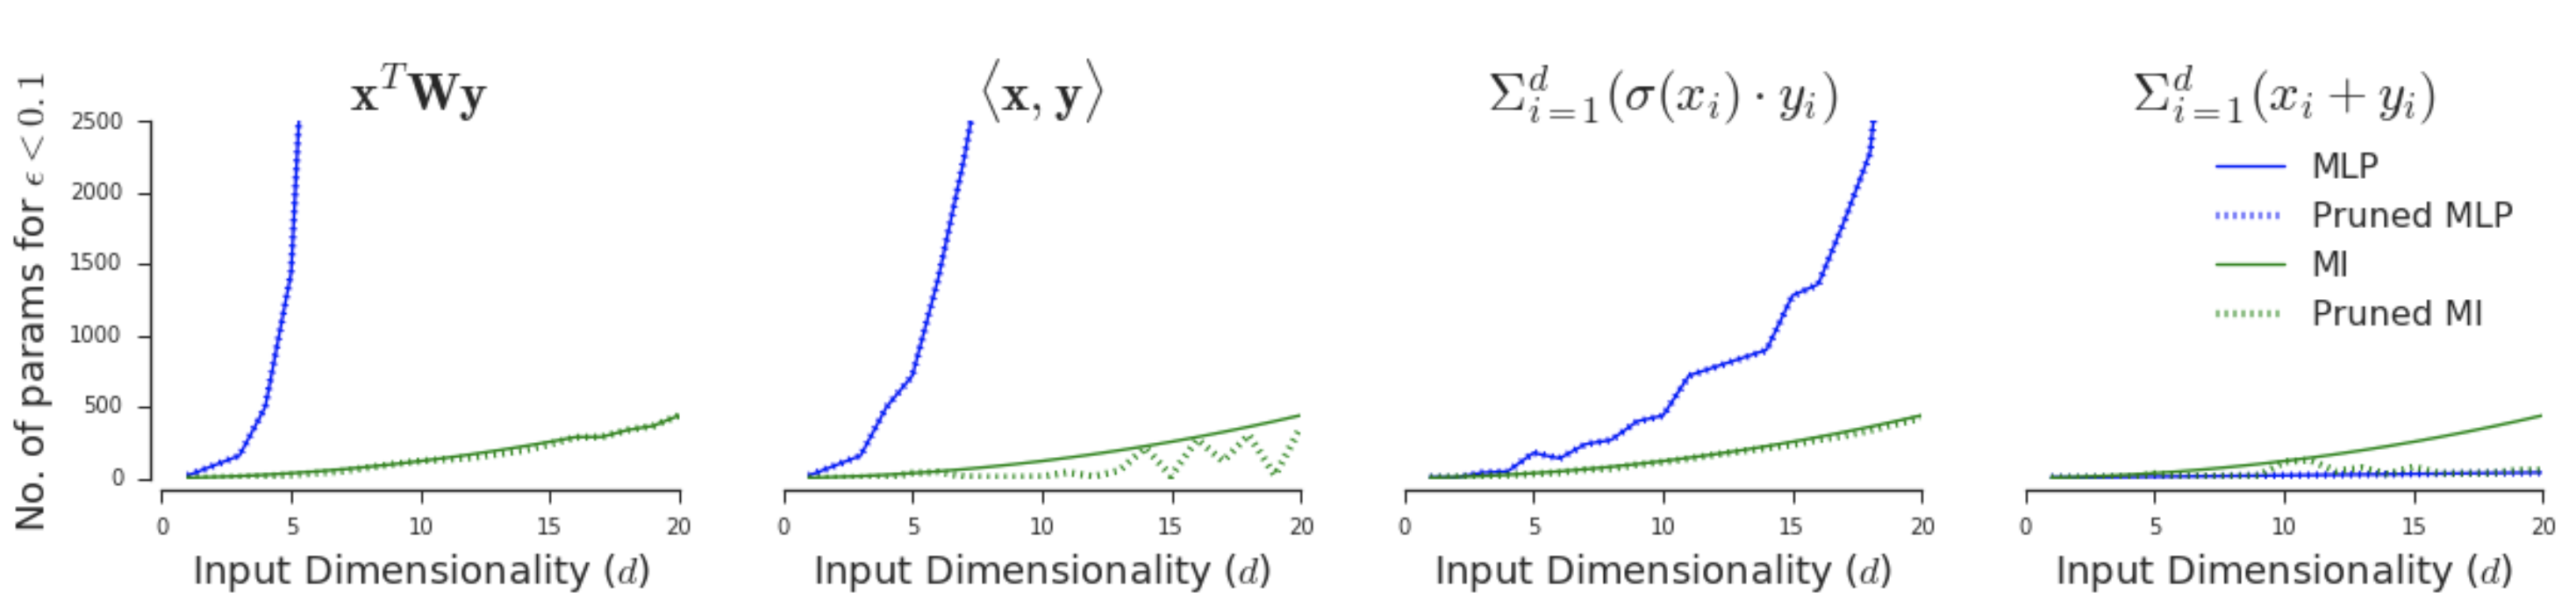
\includegraphics[width=\textwidth]{images/MIs_are_more_expressive.png}
    \end{figure}
\end{frame}

\begin{frame}{Examples of MIs}
    There are a lot of examples of MIs in the modern literature:
    \begin{figure}
        \centering
        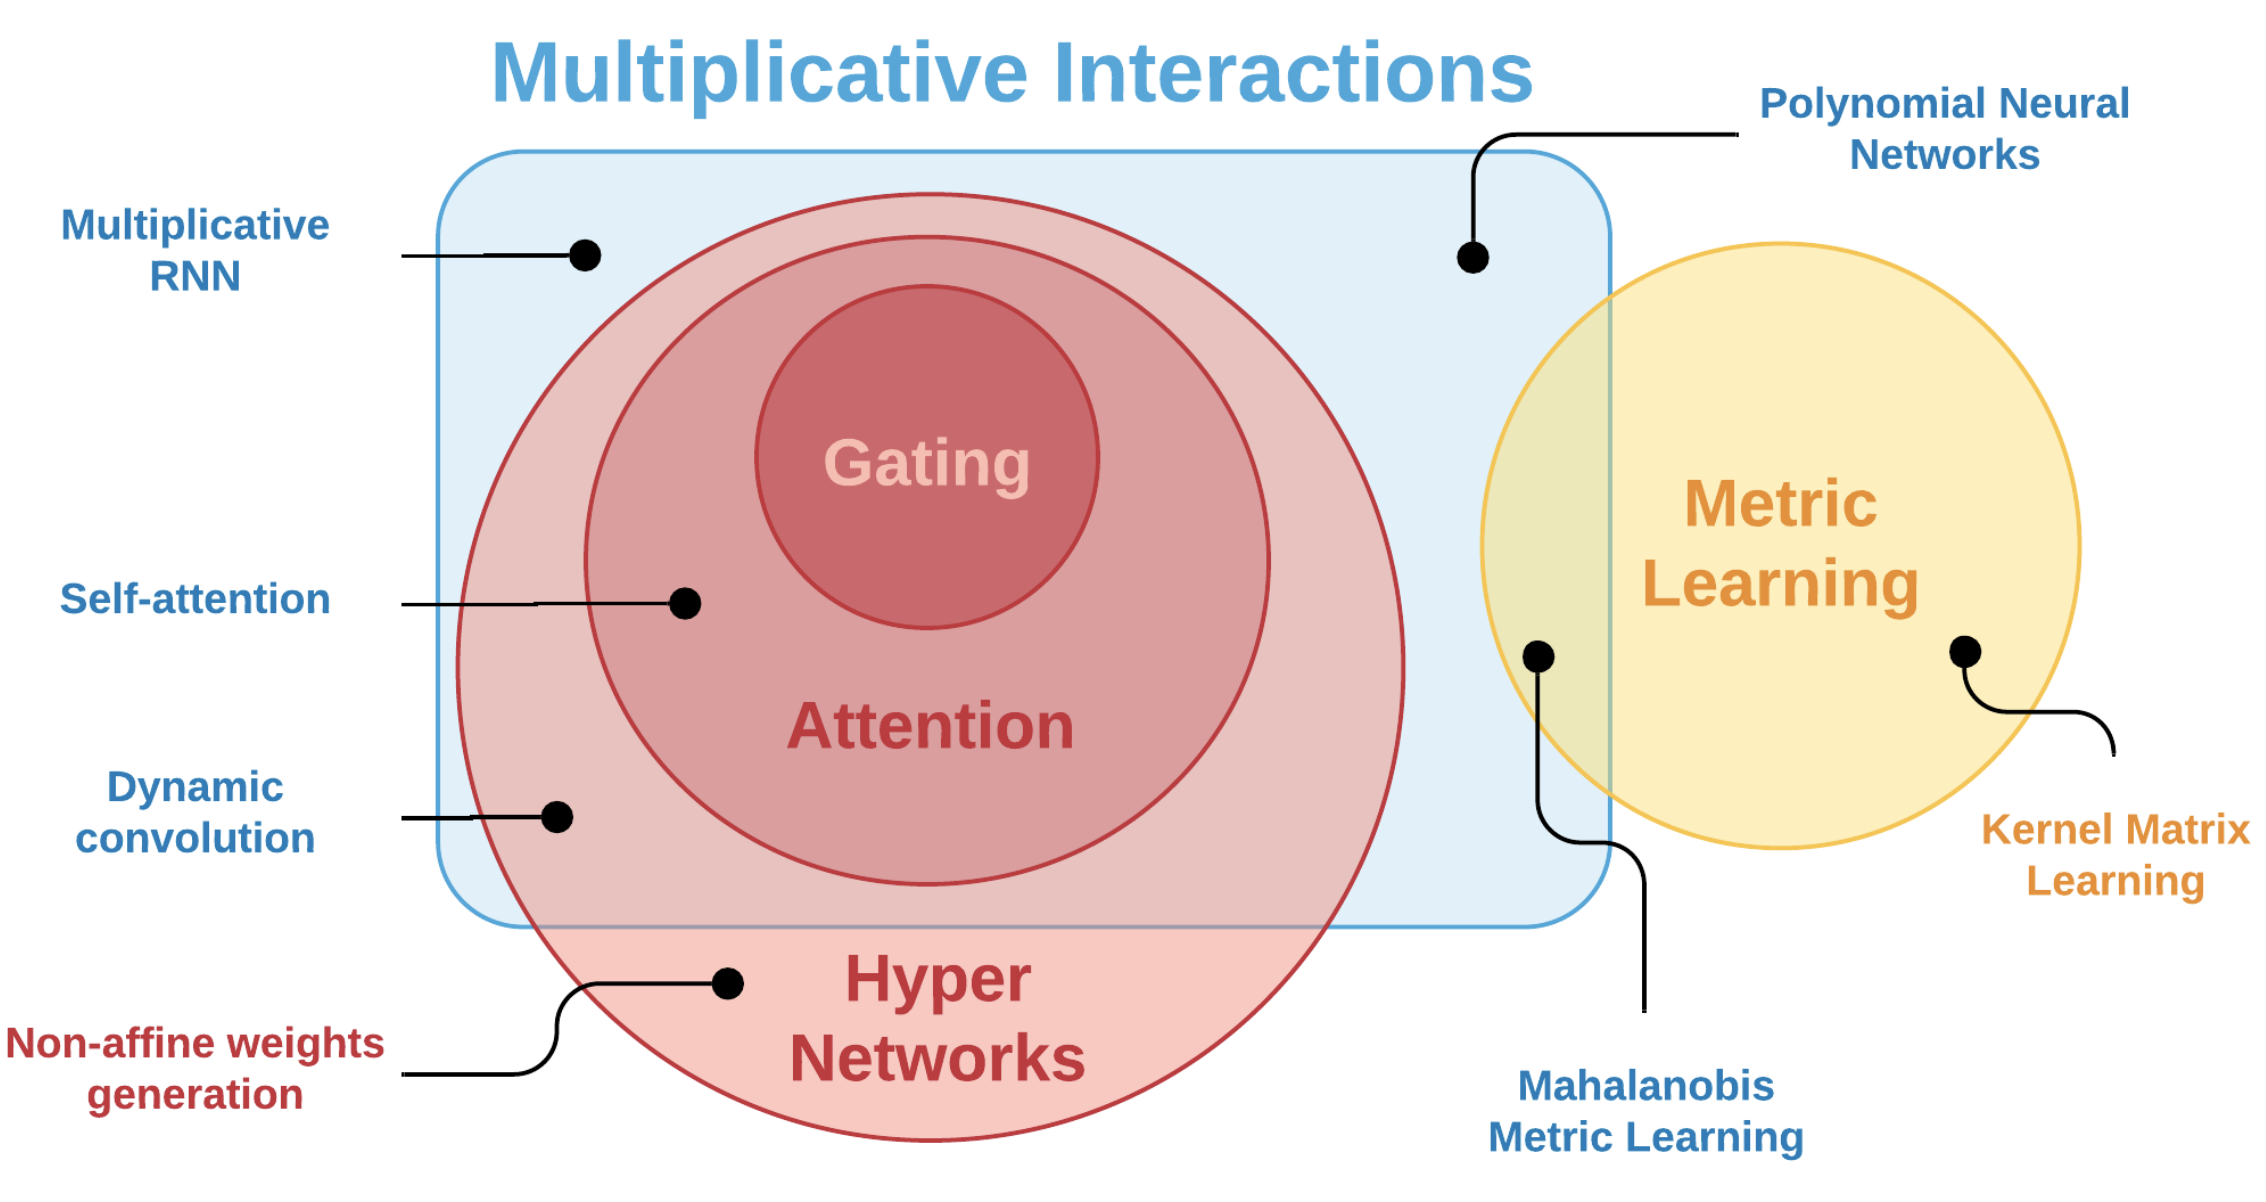
\includegraphics[width=0.8\textwidth]{images/mi_venn_diag.png}
    \end{figure}
\end{frame}

\begin{frame}{Examples of MI}
    \begin{itemize}
        \item\pause Attention can be seen as $\mathcal{M}(x, z)$:
        \begin{itemize}
            \item\pause $x$ is an input vector, we want to attend over its elements
            \item\pause we generate $m = \mathcal{M}(x,z)$ and compute $m \odot x$
            %\item\pause then $Mx$ is equivalent to $m \odot x$ where $m = \text{diag} M$.
            %\item\pause to generate a diagonal $M$ we just need to properly parametrize $\mathbb{W}, V$
        \end{itemize}
%        \item\pause Gating $a \odot x$ can be seen as $\mathcal{M}(x, z)$:
%        \begin{itemize}
%            \item\pause $\mathbb{W}$ has diagonal ``horizontal'' matrices
%            \item\pause 
%        \end{itemize}
        \item\pause Metric learning can be seen as a MI:
        \begin{itemize}
            \item\pause To have $\mathcal{M}(x,z) = z^\top x$ we just need to set $\mathbb{W}$ to ``identity'' (zeros everywhere and ones on the main diagonal)
            \item\pause More general forms of metric learning as $d_C(x,z) = (\mathbf{x}-\mathbf{z})^{T} \mathbf{C}^{-1}(\mathbf{x}-\mathbf{z})$ can be also expressed as $\mathcal{M}(x,z)$.
        \end{itemize}
        \item Hypernetworks, gating, etc
    \end{itemize}
\end{frame}

\begin{frame}{Experiment: integrate MI in LSTM}
%    \begin{itemize}
%        \item Baseline: Take vanilla LSTM with output embedding computed as $\mathbf{z}_{t+1}^{o}=\mathbf{W}_{2} \mathbf{h}_{t} +\mathbf{b}$
%        \item LSTM with MI: 
%        \item Another benifit: if $c$ is small, we need less parameters
%    \end{itemize}
    \pause In vanilla LSTM all interactions are ``concatentation''-based:
    \begin{figure}
        \centering
        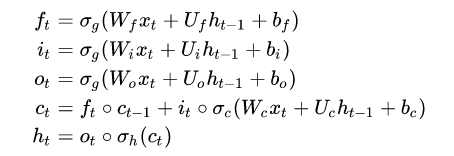
\includegraphics[width=0.6\textwidth]{images/lstm-equations.png}
    \end{figure}
    Authors replaced some of them with multiplicative ones and observed the boost in performance:
    \begin{figure}
        \centering
        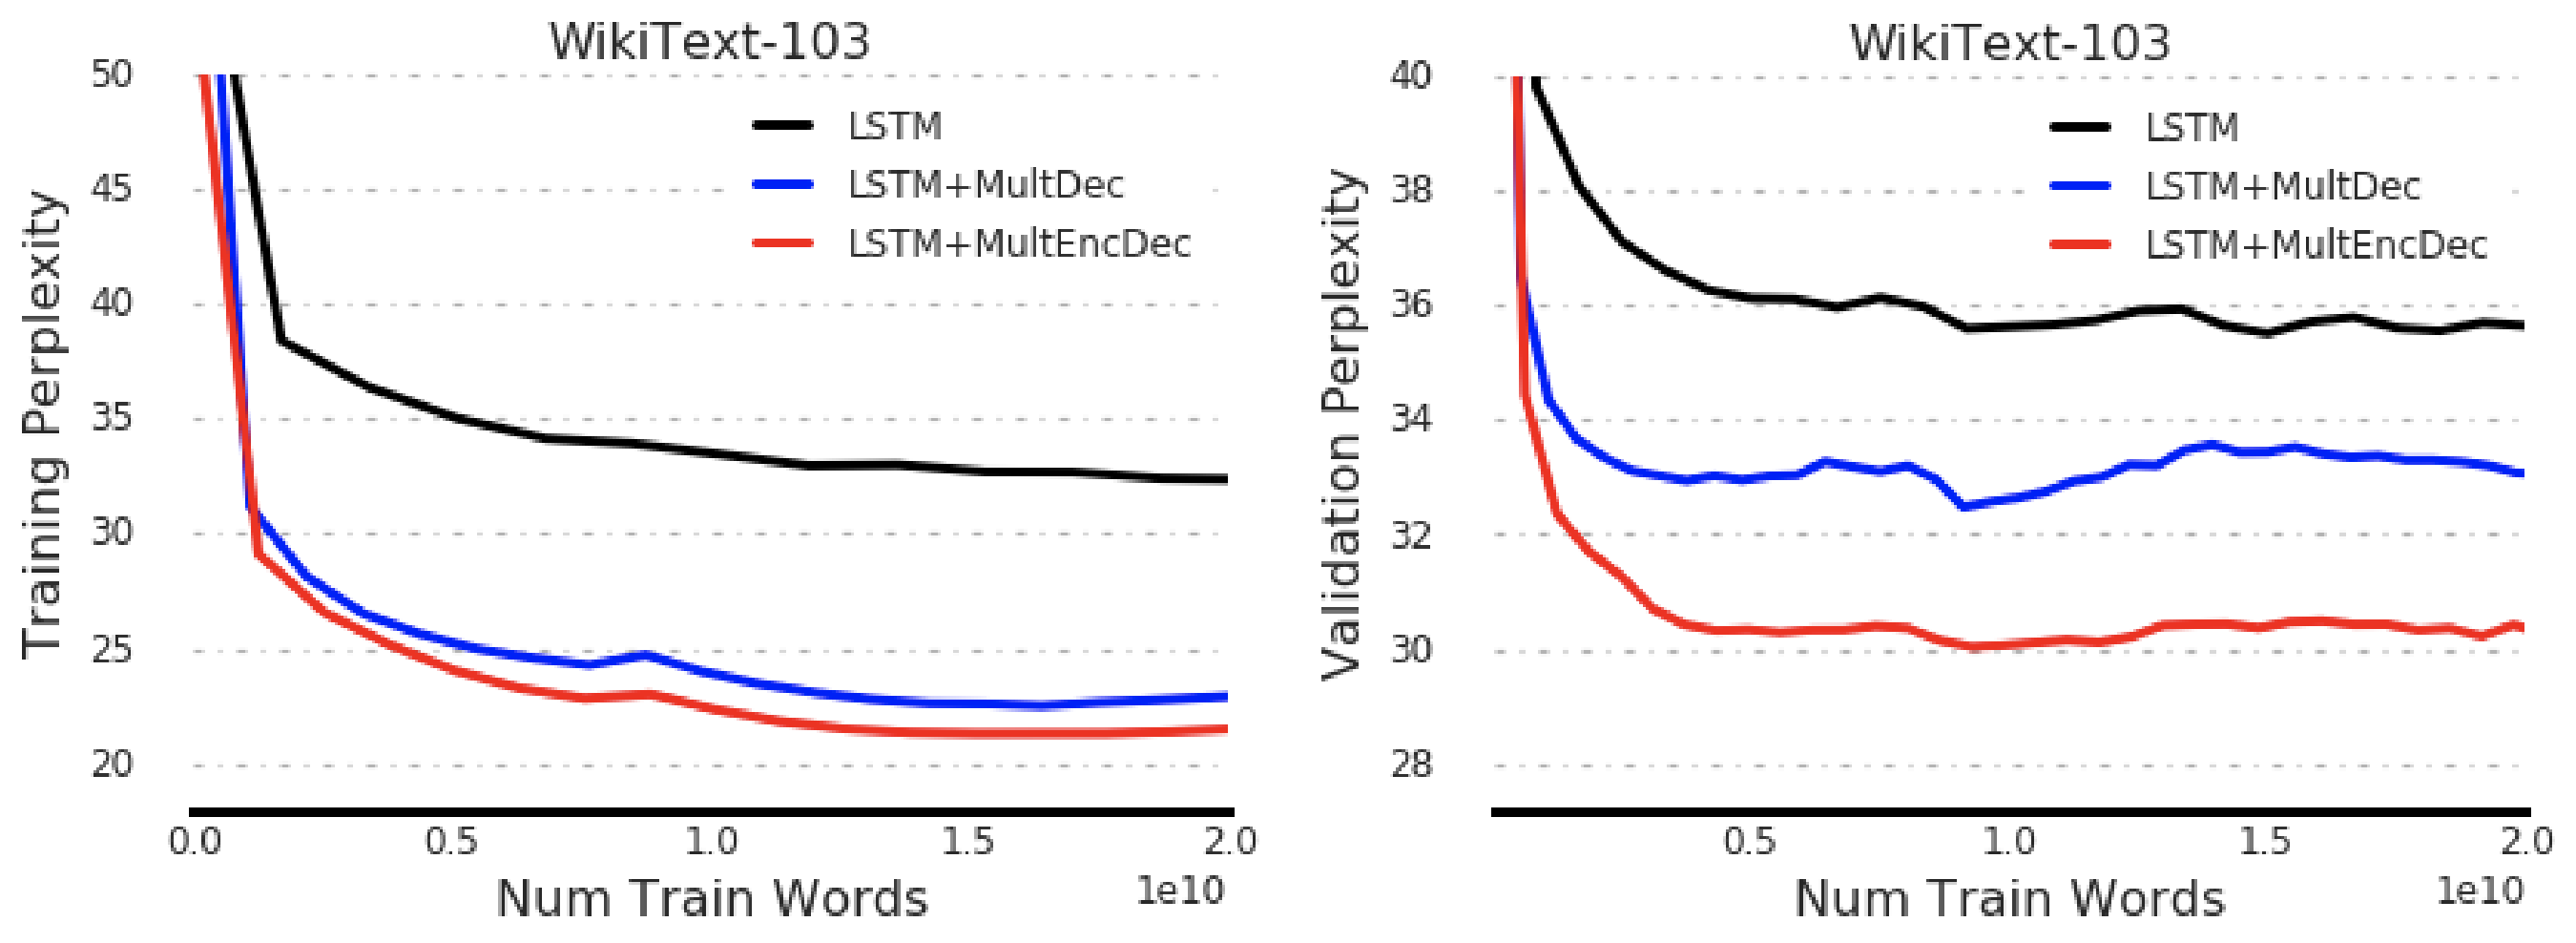
\includegraphics[width=0.9\textwidth]{images/mi-in-lm.png}
    \end{figure}
\end{frame}

\begin{frame}{Conclusion}
    \begin{itemize}
        \item Authors also did some experiments for few-shot learning and multi-task learning
        \item MI is a powerful tool to integrate different sources of information
        \item We have countless scenarios to explore them
    \end{itemize}
\end{frame}

%\begin{frame}{Examples of MIs}
%    \begin{itemize}
%        \item\pause Gating:  
%        \item\pause Hypernetworks:
%        \begin{itemize}
%            \item\pause In HN's layer $y = Wx + b$ we generate $W, b$ by another model
%            \item\pause This another model is conditioned on $z$
%            \item\pause If we generate $W, b$ via: $W = z^\top \mathbb{W} + V, b = z^\top V + b'$, then we have a MI
%        \end{itemize}
%    \end{itemize}
%\end{frame}

\end{document}
